

\section{Station de recharge}
\label{s:Recharge}

La figure \ref{f:StationRecharge} pr�sente le circuit install� sur la station de recharge. le PIC est utilis� pour g�n�rer une horloge n�cessaire au Manchester et une autre pour le hachage du signal de charge. Les signaux d'horloge ainsi que le code Manchester sont transmis au module Xbee pour ensuite �tre transmis au robot.

\begin{figure}[htp]
   \centering
   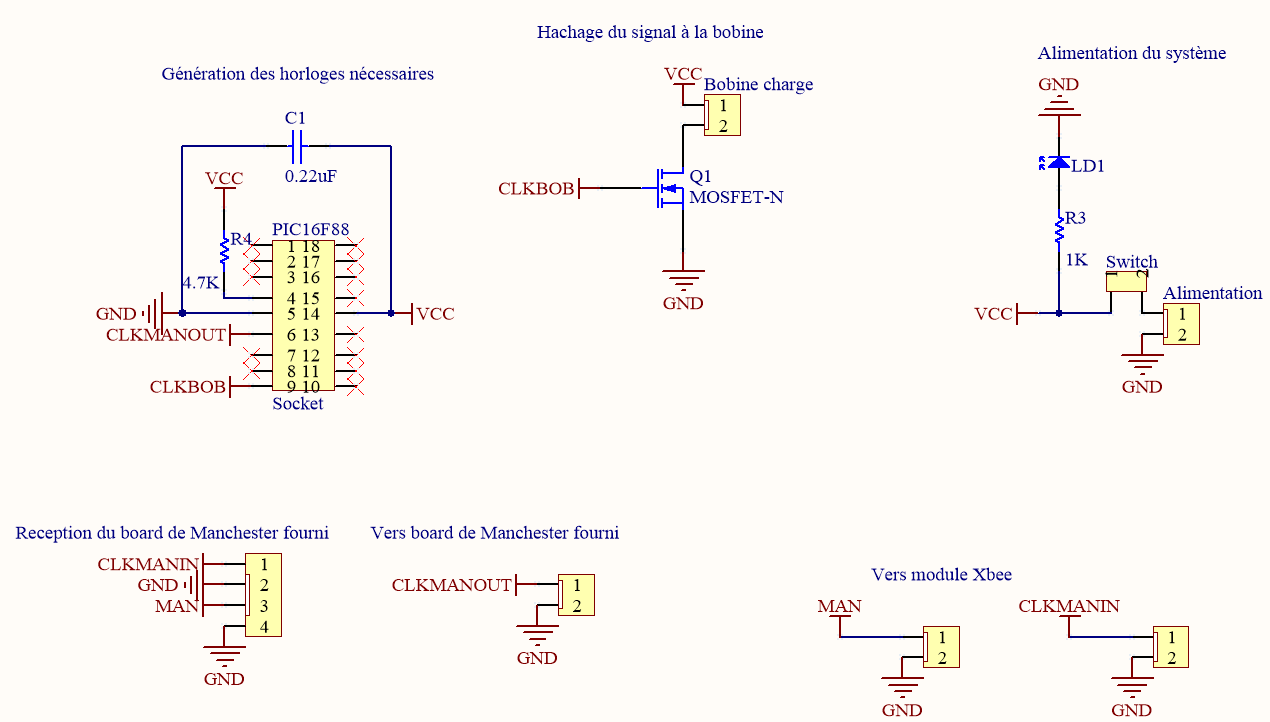
\includegraphics[width=1\textwidth]{fig/StationRecharge.png}
   \caption{Sch�ma �lectrique de la station de recharge}
   \label{f:StationRecharge}
\end{figure}

\pagebreak

\section{Circuit de charge et de d�charge du condensateur}
\label{s:Condensateur}

La figure \ref{f:Condensateur} pr�sente le circuit de charge et de d�charge du condensateur. Le MOSFET et utilis� en envoyant un PWM � sa base afin de r�duire l'effet de l'induction r�manente � l'�lectroaimant. Un interrupteur permet aussi de connecter une r�sistance permettant de d�charger les condensateurs.

\begin{figure}[htp]
   \centering
   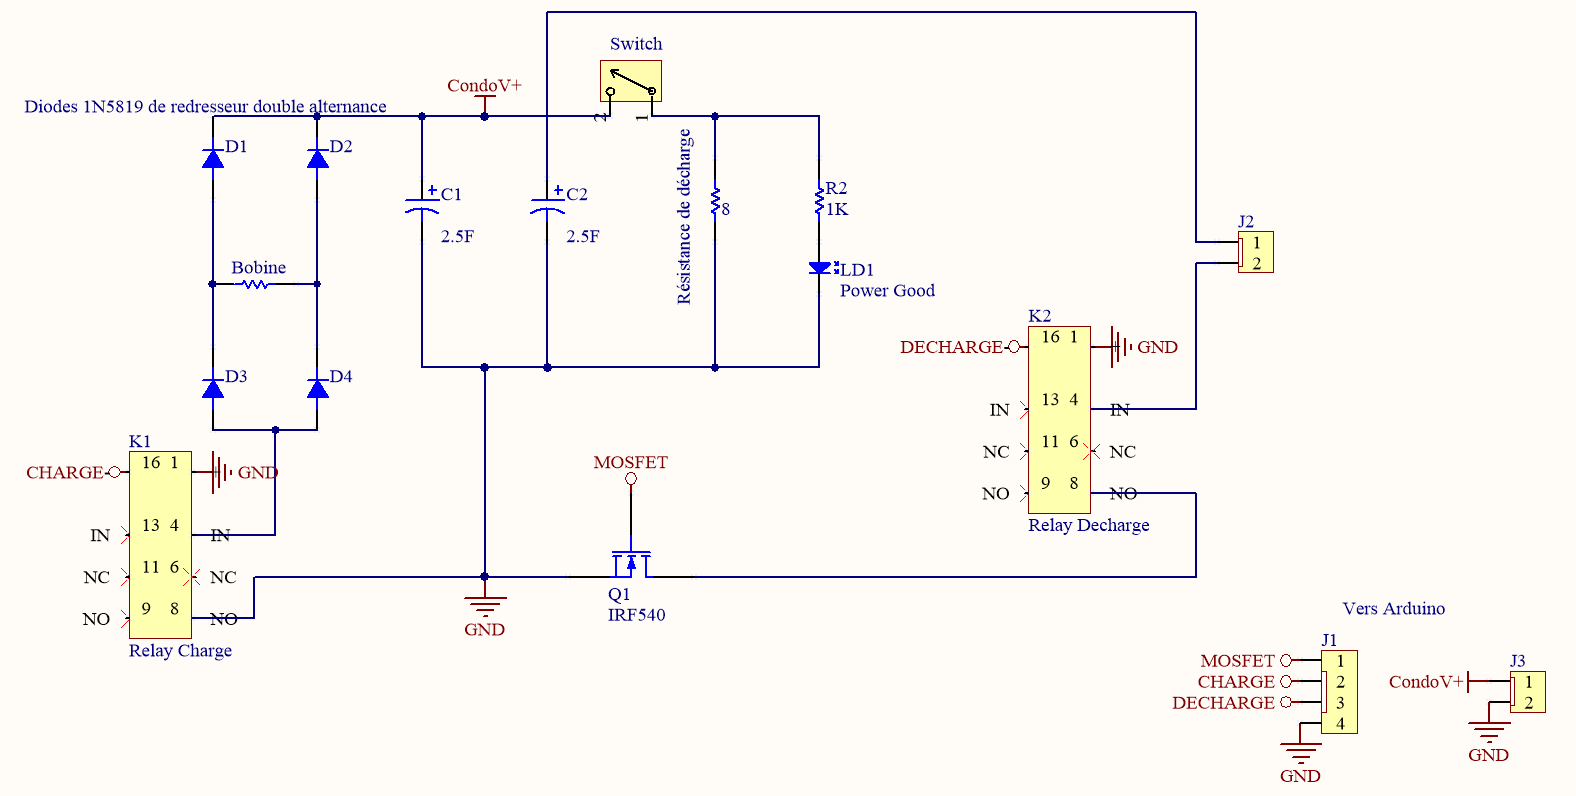
\includegraphics[width=1\textwidth]{fig/Condensateur.png}
   \caption{Sch�ma �lectrique de la charge et la d�charge du condensateur}
   \label{f:Condensateur}
\end{figure}

\pagebreak

\section{Circuit de connexions pour les moteurs}
\label{Connexions}

\subsection{Connexions moteurs et pont en H}
\label{Moteurs}

La figure \ref{f:Connexions} pr�sente le circuit de connexion utilis� pour les connections des encodeurs des moteurs et du pont en H. On utilise ce circuit situ� sous le robot afin d'�viter de rallonger les fils des moteurs et de mieux organiser les fils.

\begin{figure}[htp]
   \centering
   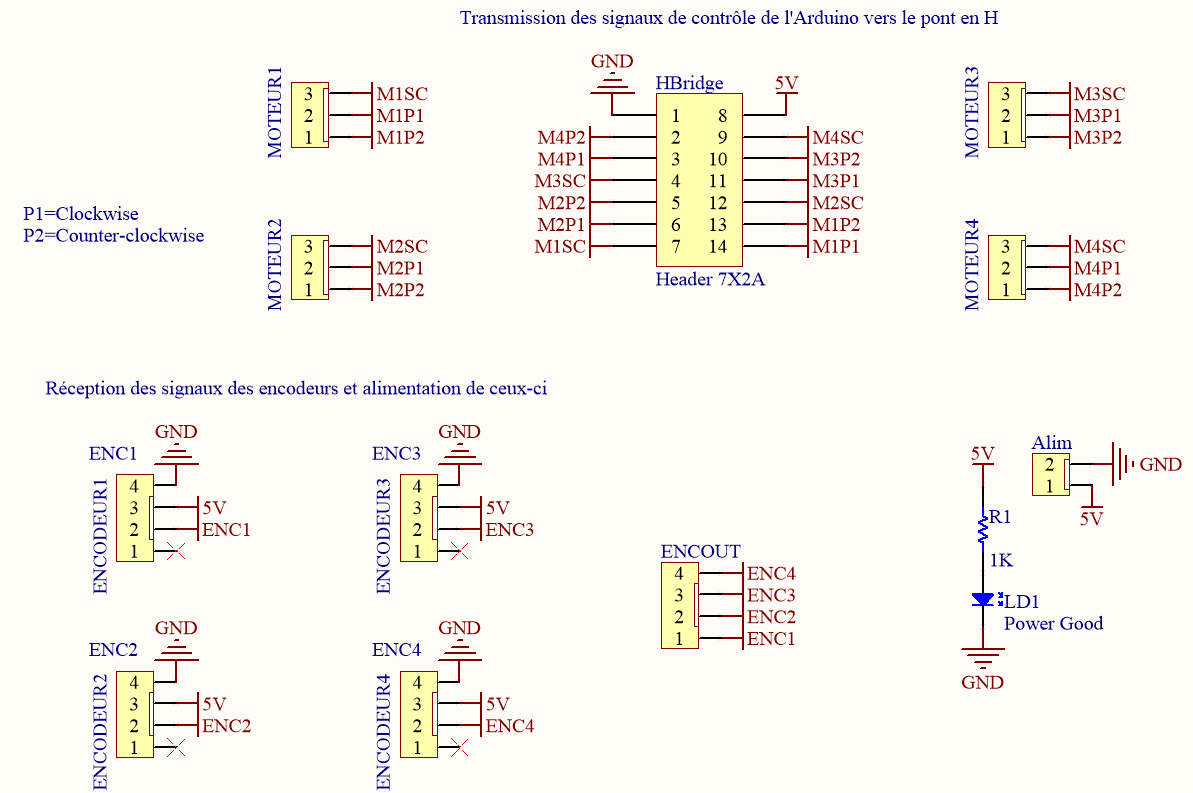
\includegraphics[width=1\textwidth]{fig/Connections.png}
   \caption{Sch�ma �lectrique du circuit de connexions des moteurs}
   \label{f:Connexions}
\end{figure}

\pagebreak

\subsection{Connexions sur l'Arduino}
\label{Arduino}

La figure \ref{f:Arduino} pr�sente les connexions de tout les syst�mes sur l'Arduino.

\begin{figure}[htp]
   \centering
   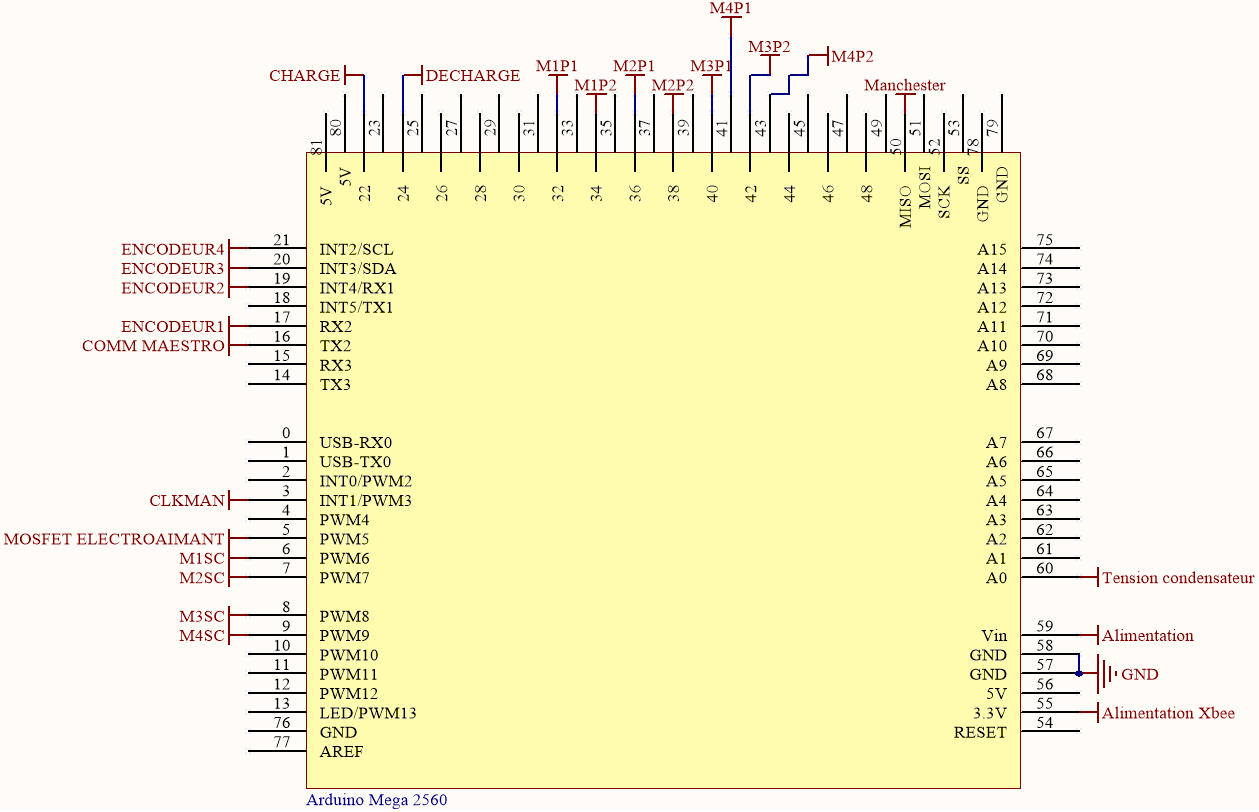
\includegraphics[width=1\textwidth]{fig/Arduino.png}
   \caption{Sch�ma des connexions sur l'Arduino Mega}
   \label{f:Arduino}
\end{figure}


\pagebreak